\documentclass[answers]{exam}

% ------------------------------------------------------------------------------ %
% -----------------------      Base for every .tex file   ---------------------- %
% ------------------------------------------------------------------------------ %

\usepackage[dvipsnames]{xcolor}
\usepackage{mathtools}
\usepackage{amssymb}
\usepackage{amsthm}
\usepackage{amsmath}
\usepackage{framed}
\usepackage{wasysym}
\usepackage{geometry}
\usepackage{cancel}
\usepackage{blindtext}
\usepackage{pgfplots}
\usepackage{graphicx}
\usepackage{lastpage}
\usepackage[most]{tcolorbox} 
\usepackage{multicol}
\usepackage{soul}
\usepackage{listings}
\usepackage{algorithm}
\usepackage{algorithmic}
\usepackage{booktabs}
\usepackage{tikz}
\usepackage{pifont}

% Libraries
\usetikzlibrary{shapes,shapes.geometric, positioning, arrows}

\geometry{%
	left=15mm,
	right=15mm,
	top=25mm,
	bottom=25mm,
	bindingoffset=0mm,
	headheight=30pt,% output from geometry tells you what this needs to be set to as a minimum
}

% Header and Footer
\pagestyle{headandfoot}
\firstpageheadrule
\runningheadrule
\firstpageheader{Convex Optimization}{\today}{Jonathan Schnell}
\runningheader{Convex Optimization}{}{Jonathan Schnell}
\firstpagefooter{}{Page \thepage\ of \numpages}{}
\runningfooter{}{Page \thepage\ of \numpages}{}

% Commands
\newcommand{\imp}[1]{\ul{\textbf{#1}}}
\newcommand{\dproduct}[1]{\left\langle #1 \right\rangle}
\newcommand{\norm}[1]{\left\lVert #1 \right\rVert}
\renewcommand{\vector}[1]{\begin{pmatrix} #1 \end{pmatrix}}
\newcommand{\abs}[1]{\left| #1 \right|}
\newcommand{\floor}[1]{\lfloor #1 \rfloor}
\newcommand{\ceil}[1]{\lceil #1 \rceil}
\newcommand{\fracpart}[2]{\frac{\partial #1}{\partial #2}}
\newcommand{\set}[2]{\left\{#1 \ \middle|\ #2\right\}}
\renewcommand{\hat}[1]{\widehat{#1}}

\newcommand{\Ker}{\operatorname{Ker}}
\renewcommand{\Im}{\operatorname{Im}}
\renewcommand{\Re}{\operatorname{Re}}
\renewcommand{\dim}{\operatorname{dim}}
\renewcommand{\div}{\operatorname{div}}
\newcommand{\rot}{\operatorname{rot}}
\newcommand{\grad}{\operatorname{grad}}
\newcommand{\vol}{\operatorname{vol}}
\newcommand{\supp}{\operatorname{supp}}
\renewcommand{\div}{\operatorname{div}}
\newcommand*{\vertbar}{\rule[-1ex]{0.5pt}{2.5ex}}
\newcommand*{\horzbar}{\rule[.5ex]{2.5ex}{0.5pt}}

\theoremstyle{definition}
\newtheorem*{definition}{Definition}
\newtheorem*{beispiel}{Beispiel}
\newtheorem*{remark}{Remark}

\theoremstyle{plain}
\newtheorem*{proposition}{Proposition}
\newtheorem*{satz}{Satz}
\newtheorem*{korollar}{Korollar}
\newtheorem*{lemma}{Lemma}
\newtheorem*{theorem}{Theorem}


% Quote
\newtcolorbox{zitat}[1]{%
	colback=lightGray,
	grow to right by=-10mm,
	grow to left by=-10mm, 
	boxrule=0pt,
	boxsep=0pt,
	breakable,
	enhanced jigsaw,
	borderline west={4pt}{0pt}{gray},
	#1
}

% Use colors in equations
\newcommand{\highlight}[2]{\colorbox{#1}{$#2$}}%
\definecolor{lightGray}{gray}{0.9} 

% To add shortcut of script Letters in Equations
\newcommand{\s}[1]{\mathcal{#1}}
\newcommand*\circled[1]{\tikz[baseline=(char.base)]{
            \node[shape=circle,draw,inner sep=2pt] (char) {#1};}}
\newcommand{\cmark}{\ding{51}}
\newcommand{\xmark}{\ding{55}}


\newenvironment{claim}[1]{
		\par\noindent
		\textbf{Claim.} #1
		\begin{tcolorbox}[blanker, top=3mm, bottom=3mm, left=3mm, borderline west={1pt}{0mm}{black}]
		\noindent\textit{Proof of Claim.} 
}{
	\hfill$\blacksquare$	
	\end{tcolorbox}\noindent
}

% To add shortcut of number's set Z
\newcommand*{\Z}{\mathbb{Z}}
\newcommand*{\N}{\mathbb{N}}
\newcommand*{\R}{\mathbb{R}}
\newcommand*{\Q}{\mathbb{Q}}
\newcommand*{\C}{\mathbb{C}}
\newcommand*{\F}{\mathbb{F}}
\newcommand*{\K}{\mathbb{K}}

% To add shortcut of empty set
\renewcommand*{\o}{\varnothing}
\pgfplotsset{compat=1.9}

\everymath{\displaystyle}

% Line-Height
\linespread{1.15}

\graphicspath{{Files/}}

% ------------------------------

\begin{document}

	$ $
	\begin{center}
		\huge \textbf{Exercise session notes - Week 4}  \\ \vspace*{3mm}
        \Large{Support Vector Machine + Duality}
	\end{center}
	$ $\\

    \section{Support Vector Machine}

    We first review the definition of a Support Vector Machine (SVM). 
    \paragraph*{Definition.}
        \textbf{Support Vector Machine} \\
        \underline{Input.} points $x_1,\ldots, x_m\in \R^n$ with labels $y_1,\ldots, y_m\in \{-1,1\}$. \\ 
        \underline{Output.} Hyperplane $(w, b)$ separating points with different labels, i.e.
        \begin{align*}
            w^\top x_i + b \geq 1 \quad&\forall i \text{ with } y_i = 1 \\ 
            w^\top x_i + b \leq -1 \quad&\forall i \text{ with } y_i = -1
        \end{align*}
        maximizing the margin between the set of points.
    \begin{center}
        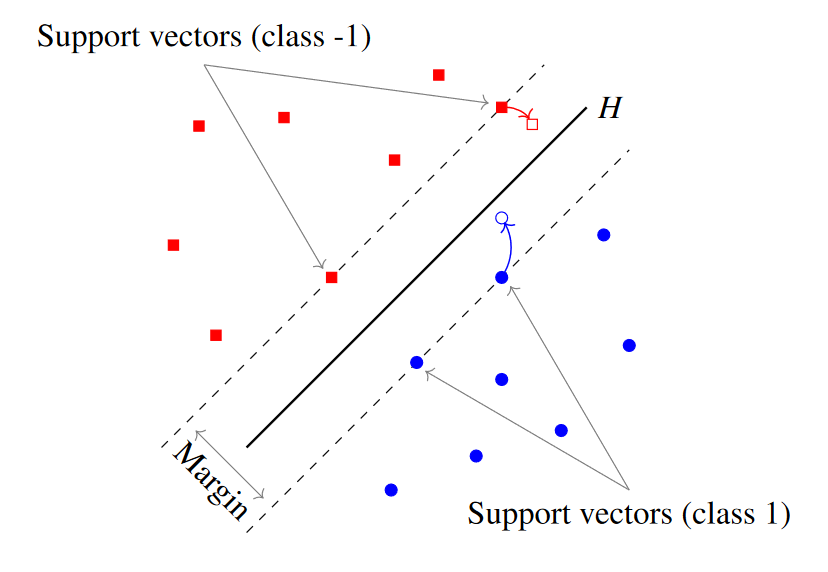
\includegraphics[width=0.4\textwidth]{SVM.PNG}
    \end{center}

    In the lecture we saw that if the points are linearly separable, then the margin is given by $\tfrac{2}{\norm{w}}$. Therefore we can model the problem as the following convex program.
    \begin{alignat*}{3}
        \min\quad\quad \norm{w}^2& && \leftarrow \text{convex objective}\\ 
        y_i(w^\top x_i + b) &\geq 1 &&\leftarrow \text{linear constraint}\\ 
        w,b&\text{ free}\quad\quad &&
    \end{alignat*}
    Often the set of points is not linearly separable, and in this case we can make use of Feature Maps. Assume we have the following set of points
    \begin{center}
        \includegraphics*[width=0.3\textwidth]{FeatureMaps.PNG}
    \end{center}
    Note that these points are not linearly separable but we see that the crosses are concentrated within some range and circles are outside of that range. Therefore we apply the feature map $(x,y)\mapsto (x,y, x^2+y^2)$ and obtain a new set of points that are now linearly separable and we can apply the SVM algorithm.
    \begin{center}
        \includegraphics*[width=0.4\textwidth]{FeatureMaps2.PNG}
    \end{center}
    Note that although there always exists a feature map that makes the points linearly separable it is usually very hard to find one.

    \section{Duality}
    Given is a \underline{general} mathematical program (P)
    \begin{align*}
        \min\set{f(x)}{g_i(x)\leq 0,\ h_j(x) = 0}
    \end{align*}
    For such a program we define the \imp{Lagrangian} 
    $$ L(x,\lambda, \nu) = f(x) + \sum \lambda_i g_i(x) + \sum \nu_j h_j(x) $$
    with Lagrange multipliers $\lambda_i\geq 0$, $\nu_j\in \R$. Note that the Lagrangian is affine in $\lambda, \nu$ and for any point $x$ feasible for (P) we have 
    $$ L(x,\lambda, \nu) \leq f(x) \quad\quad \text{for } \lambda\geq 0, \nu \text{ free} $$
    We define the \imp{Lagrange dual function} 
    $$ \hat{L}(\lambda, \nu) = \inf_{x}\ L(x,\lambda, \nu) $$
    and note that this function is \underline{concave} (as infimum of concave functions). Finally we define the \imp{Lagrange dual program} (D) 
    \begin{align*}
        \max\set{\hat{L}(\lambda, \nu)}{\lambda \geq 0,\ \nu \text{ free}}
    \end{align*}
    Let's do some simple calculations: For any feasible point $x$ for (P) and any feasible point $\lambda, \nu$ for (D) it holds
    \begin{align*}
        \hat{L}(\lambda, \nu)\ \leq\ L(x,\lambda, \nu)\ \leq\ f(x)
    \end{align*}
    In particular, since the the two sides of the inequality are independent, we can squash the values and we get 
    $$ \max_{\lambda, \nu}\ \hat{L}(\lambda, \nu)\ \leq\ \min_{x}\ f(x) $$
    This just says that if the two programs are feasible, the optimal value of (D) gives us a lower bound on the optimal value of (P). This property is a special case of the \underline{Weak Duality Theorem}. Moreover note that for any general mathematical program (P) its Lagrange dual program (D) is always a convex program, therefore it can be solved efficiently. In particular for any (also NP-hard) problem we can find efficiently a lower bound on the optimal value. Next week we will see the general statement of Weak Duality Theorem and the Strong Duality Theorem. 
\end{document}